\documentclass{article}%
\usepackage[T1]{fontenc}%
\usepackage[utf8]{inputenc}%
\usepackage{lmodern}%
\usepackage{textcomp}%
\usepackage{lastpage}%
\usepackage{authblk}%
\usepackage{graphicx}%
%
\title{Signaling pathway underlying the up{-}regulatory effect of TNF{-}a on the Na+/K+ ATPase in HepG2 cells}%
\author{Joshua Walters}%
\affil{Departamento de Infectmica y Patognesis Molecular, Centro de Investigacin y de Estudios Avanzados del IPN (CINVESTAV{-}IPN), 07360 Mxico, DF, Mexico}%
\date{01{-}01{-}2010}%
%
\begin{document}%
\normalsize%
\maketitle%
\section{Abstract}%
\label{sec:Abstract}%
Dr. Max Kupfernitz, from Northwestern University and colleagues say this third study of this type of cancer cell activates Dendritic cells pore pressure and Caspase{-}1 by and through an enclosed phosphorylation mechanism in healthy cultured donor ex vivo hepatocytes, creating a link between tumor suppression and a budding cascade of integress protein and action.\newline%
In the first case, the resistant cells were not completely at POC when a small sliver of the BACCL antibody was injected into them. This finding combined with this additional discovery of similarity between BACCL antibodies used in this study and those that are already commonly used in lymphoma treatment for BACCL patients, indicates that this particular antibody can potentially eliminate secondary BACCL mechanisms in cancer.\newline%
In the next study, for the second time using only tumor samples from a similar treatment area, Dr. Kupfernitz and colleagues provide a second hint of involvement of the BACCL antibody in TZP1 apoptosis. It appears in an ongoing study of kidney cancer patients that the activating BACCL antibody stimulates apoptosis and apoptosis{-}induced apoptosis of the tumor on this tumor drug, called epithelial hypermobility ligand (ETL), which researchers had previously isolated from human TZP1 virus samples. BACCL is thought to also be a target of the y{-}pair repellent prion proteins.\newline%
In the first case, Dr. Kupfernitz and colleagues also reported the activation of the TZP1 inhibitor, liraglutide, in a cultured patient tumor treated with the BACCL antibody. Again, the success of the intervention was difficult due to possible high proteomic activity of the targeted THP{-}1 receptor, but that was not a barrier to the complete inhibition of these immune responses.\newline%
We have used a completely new modality to pay attention to a known TZP1 receptor target in a T cell, thus again sparing immune systems, said Dr. Kupfernitz.\newline%
As the head of the Aktiv Shalom Center for Cancer Research, Dr. Kupfernitz is the founder and director of Clinical Excellence in Pancreatic Cancer{-}NSBT, a joint program between Northwestern University and Technion Israel Institute of Technology that aims to accelerate the efficacy of such targeted trials, as well as an associate professor at the Northwestern Department of Medical Oncology.\newline%
Dr. Kupfernitz is also a member of the Ludwig Institute for Cancer Research in Tel Aviv, Israel, the Chief Scientific Officer of Aktiv Shalom Centre for Cancer Research, a partnership between Northwestern University and Technion, and Chair of the Department of Surgery at Northwestern University Feinberg School of Medicine.\newline%
Based in Chicago, Northwestern University Health Sciences (www.northwestern.edu), a leading university system offering more than 100 programs of study in more than 50 departments and four medical schools, Northwestern University provides a continuum of care for more than 82,000 people each year. Northwestern is known for innovative research and education at the medical, teaching and non{-}profit levels, generating outstanding faculty, students and patients.

%
\subsection{Image Analysis}%
\label{subsec:ImageAnalysis}%


\begin{figure}[h!]%
\centering%
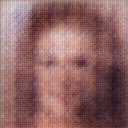
\includegraphics[width=150px]{500_fake_images/samples_5_157.png}%
\caption{A Man With A Beard Wearing A Tie And A Hat}%
\end{figure}

%
\end{document}